%
%  Chapter:  2 - Nuclear Models for High Spin Phenomena
%  Modified: 2/16/2015
%  Author:   James Till Matta
%
%%%%%%%%%%%%%%%%%%%%%%%%%%%%%%%%%%%%%%%%%%%%%%%%%%%%%%%%%%

\chapter{NUCLEAR MODELS FOR HIGH SPIN PHENOMENA}
\label{chp:models}
The atomic nucleus, discovered in $1911$ by Ernest Rutherford\cite{rutherfordNuclearModel}, is a tiny point of matter at the heart of an atom. This point of matter, is approximately $1-10fm$ across, contains more than $99.94\%$ of an atom's mass, and is composed of protons and neutrons. Since its discovery the nucleus has been studied and characterized using ever more sophisticated models.

\section{Introduction}
\label{sec:models-into}

Examination of the two proton and two neutron separation energies (Fig \ref{fig:chp2-masses}) shows several distinct discontinuities at specific numbers of protons and neutrons.. Examination of the energies of the first $2^+$ (Fig \ref{fig:chp2-two-plus-energies}) states show peaks at the same numbers of protons. These ``Magic Numbers'' occur at numbers of protons and neutrons where there is a dramatic increase in the nucleus' stability. By analogy to atomic theory these magic numbers are construed to be closures of major shells. From this we conclude that the nucleus has shell structure which leads to the shell model of the nucleus.
\begin{figure}
\label{fig:chp2-masses}
\centerline{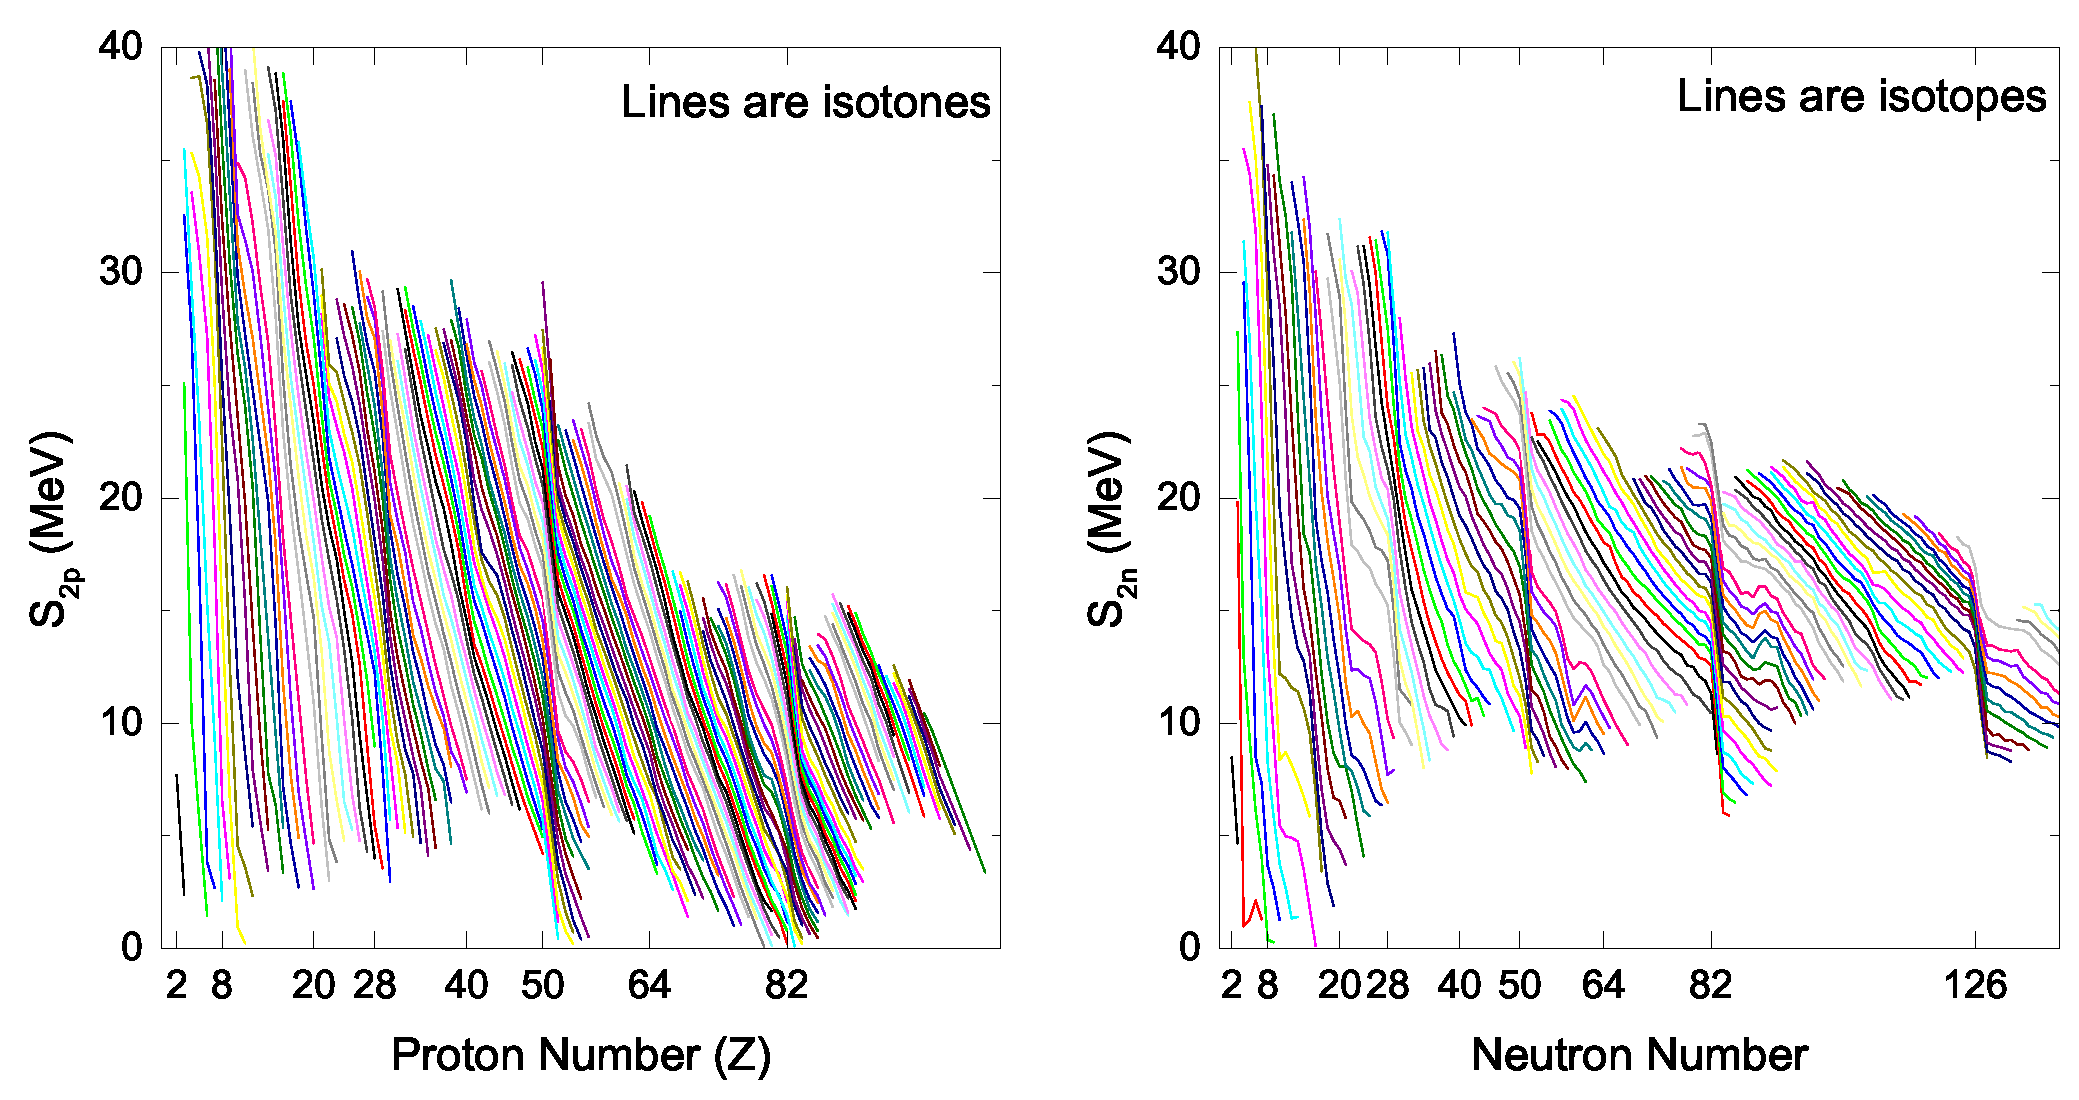
\includegraphics[height=0.3\textheight]{./img/c2/2nuc_sep_en.eps}}
	\caption{Left: Two proton separation energies plotted versus proton number. Each line is a set of isotones. Right: Two neutron separation energies plotted versus neutron number. Each line is a set of isotopes. Values calculated from: Ref.\cite{AME20031,AME20032}}
\end{figure}

\begin{figure}
\label{fig:chp2-two-plus-energies}
\centerline{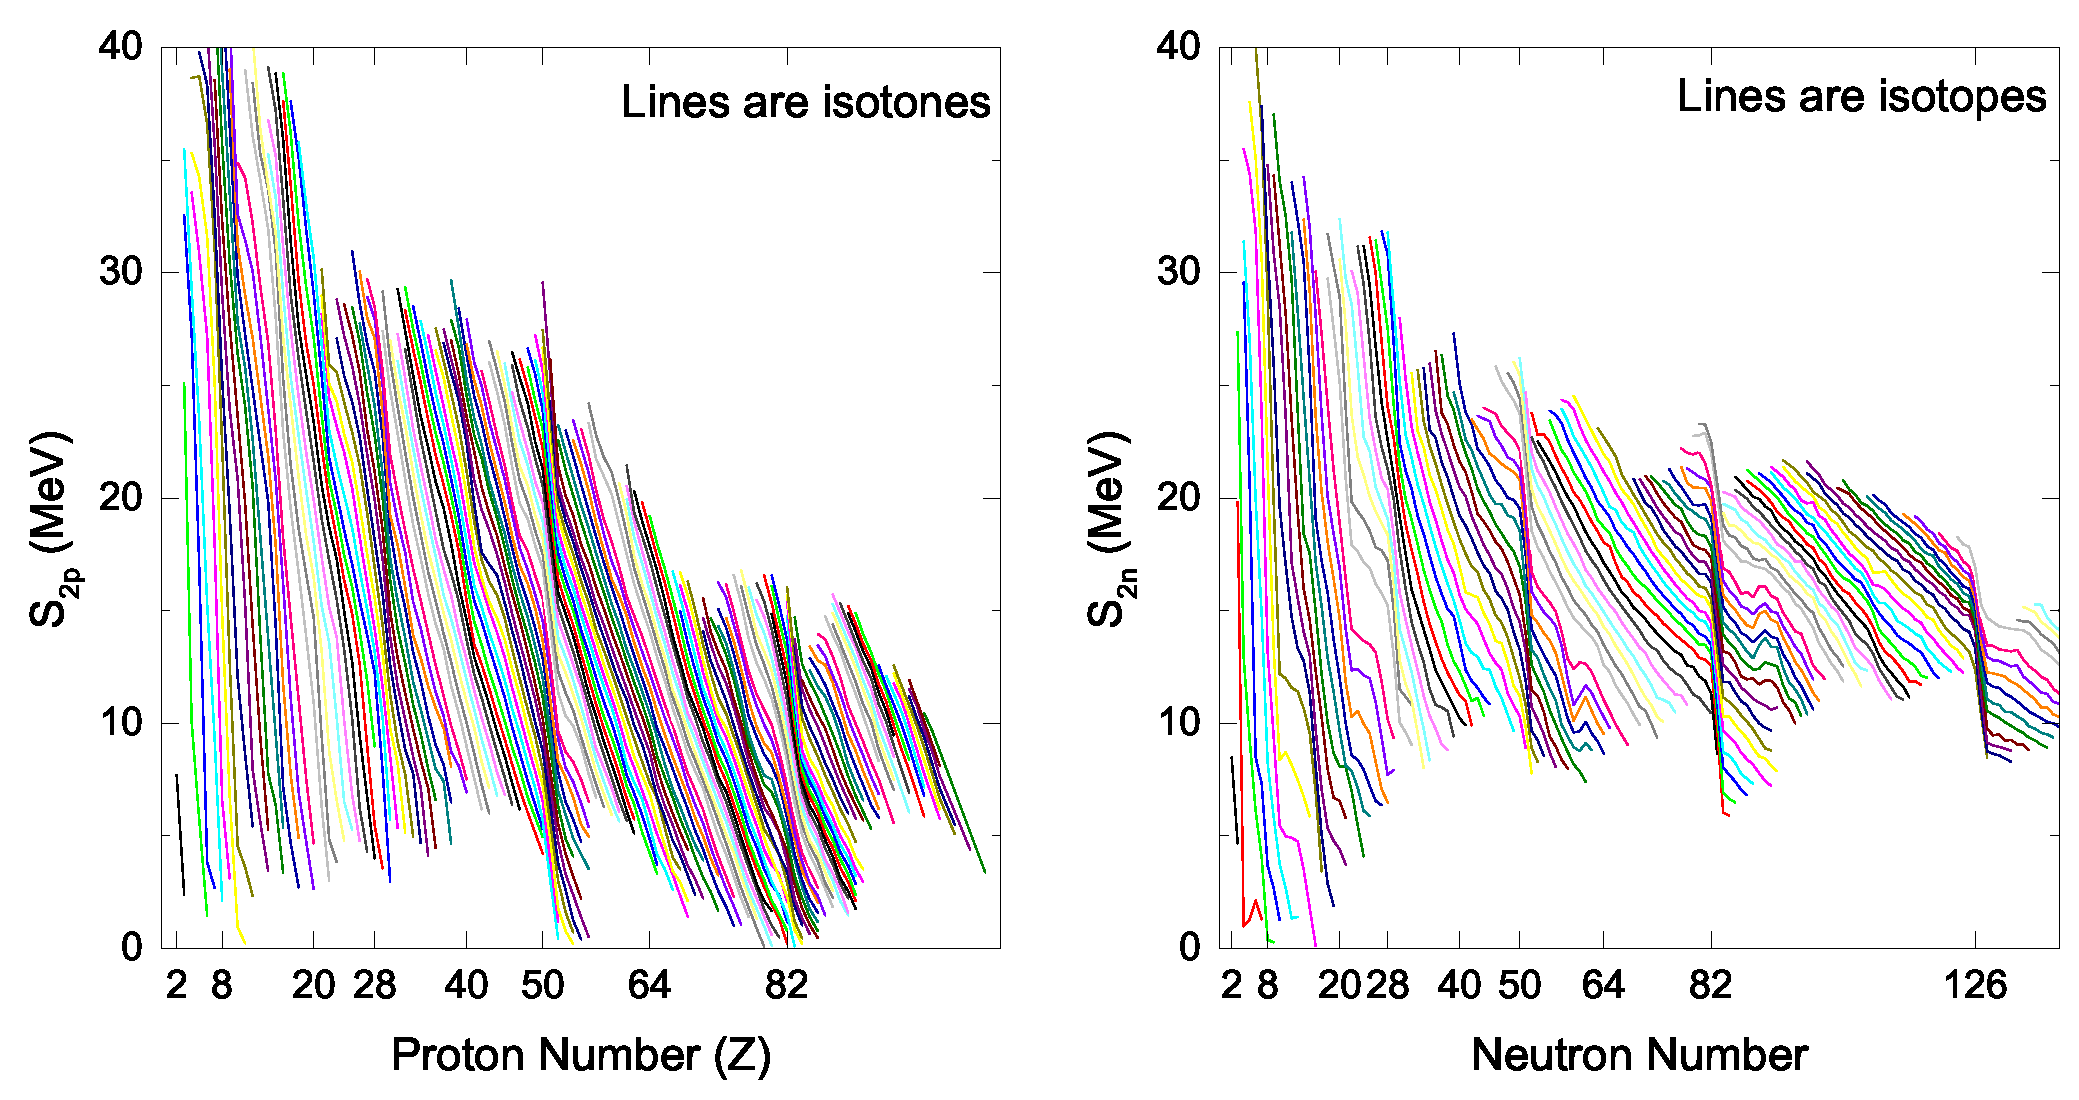
\includegraphics[height=0.3\textheight]{./img/c2/2nuc_sep_en.eps}}
	\caption{Left: First excited $2^+$ energies plotted versus proton number. Each line is a set of isotones. Right: First excited $2^+$ energies plotted versus neutron number. Each line is a set of isotopes. Figures adapted from: Ref.\cite{RamanTwoPlus}}
\end{figure}

\section{The Shell Model}
\label{sec:models-shell-model}
\subsection{The Deformed Shell Model}
\label{ssec:models-shell-model-def-sm}
\section{Rigid Rotor Model}
\label{sec:models-rigid-rotor}

\section{Tilted Axis Cranking}
\label{sec:models-tac}

\section{Wobbling Vibrations in Nuclei}
\label{sec:models-wobbling}
\subsection{Quasiparticle Triaxial Rotor (QTR)}
\label{sec:models-qtr}
\subsection{Signatures of Wobbling}
\label{sec:models-sig}
